%!TEX root = A0.Master.tex
\chapterbegin{Tecnologías y herramientas empleadas}
En este capítulo se detallan las tecnologías que se han empleado para la realización de este proyecto, así como las herramientas software utilizadas, su elección frente a otras alternativas y la labor para la que fueron utilizadas en el ámbito del proyecto.

\section{iOS}
Creado para un hardware en concreto, iOS se ha convertido, en cuanto a software, en la pieza central de Apple desde el año 2007. Actualmente es el núcleo de todos los dispositivos móviles de la compañía: iPhone, iPod Touch y iPad, e incluso de los últimos modelos de Apple TV.

En su lanzamiento, una de las grandes bazas de este Sistema Operativo fue el uso de la tecnología \emph{Multi-Touch}, que permite la manipulación de los objetos en pantalla mediante acciones o \emph{gestos}, tales como \emph{pellizcar}, \emph{tocar} o \emph{deslizar}. Esto produjo un cambio en el paradigma móvil, haciendo que los terminales con teclados físicos hayan ido desapareciendo y, a su vez, el mercado se inunde de \emph{smartphones}, todos ellos con su tienda de aplicaciones.

Las aplicaciones para terceros para iOS aparecieron en marzo de 2008, cuando Apple anunció el lanzamiento del SDK para iOS, así como la \emph{App Store}, la plataforma donde los desarrolladores pueden publicar y comercializar sus aplicaciones diseñadas para iPhone, iPod Touch, iPad, Mac OS X y Apple Watch.

iOS usa una arquitectura en 4 capas, de las cuales las 3 primeras son compartidas con OS X (aunque optimizadas): \emph{Core OS}, \emph{Core Services}, \emph{Media} y \emph{Cocoa Touch}.

\begin{figure}[h]
	\centering
		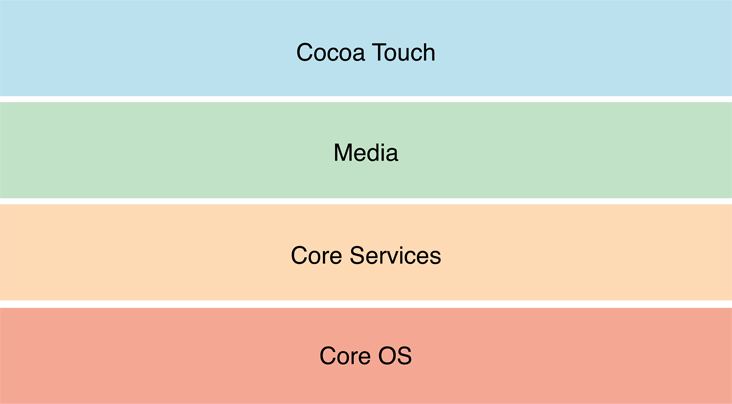
\includegraphics[width=0.5\textwidth]{./img/ios-layers.png}
	\caption{Capas de iOS}
\end{figure}

\subsection*{Core OS}
Contiene los frameworks más básicos para el funcionamiento del Sistema Operativo. Entre ellos podemos encontrar: Core Bluetooth, Network Extension, Security o System.

\subsection*{Core Services}
Contiene los sistemas fundamentales para las aplicaciones. En esta capa podemos acceder a servicios tan imprescindibles en algunas apps como Core Foundation (gestión de hilos, cadenas de caracteres, parseado de documentos XML, manipulación de URLs, etc.), Core Media, Core Location, CFNetwork, Address Book, JavaScript Core, Social, WebKit, etc.

\subsection*{Media}
Contiene todo lo relacionado con audio, vídeo, texto y gráficos. AV Foundation, AV Kit, Core Audio, Core Graphics, Core Text, GLKit, Image I/O o Metal son algunos de los frameworks disponibles en esta capa.

\subsection*{Cocoa Touch}
Siendo la última capa de iOS, su propósito es el de ofrecer todos los recursos para hacer posible la interacción del usuario con las aplicaciones: gráficos, botones y gestos. Algunos de los frameworks en esta última capa son: MapKit, PushKit, Notification Center y UIKit. Éste último puede ser considerado el más importante de esta capa, ya que incorpora todos los elementos básicos de una app, incluyendo su infraestructura, al contener el bucle principal de la aplicación.

\subsection{iPhone OS 1.0, 29 de junio de 2007}
La primera versión de este Sistema Operativo nunca tuvo un nombre definido. Con la salida al mercado del iPhone original, en junio de 2007, el equipo de márketing de Apple únicamente mencionaba que este dispositivo utilizaba una versión simplificada de OS X.

Justo antes de la salida al mercado se anunció que el iPhone únicamente permitiría aplicaciones web desarrolladas por terceras partes, con apenas acceso a diversos sistemas del dispositivo como el hacer una llamada o mandar un correo electrónico \cite{iPhoneWebApps}.

Fue ya en marzo de 2008, con la publicación por parte de Apple del SDK, cuando la compañía empezó a usar el término \emph{iPhone OS} para referirse al Sistema Operativo del iPhone. Gracias a este SDK, terceras partes podrían desarrollar aplicaciones para iPhone y distribuirlas a través de la plataforma exclusiva para iPhone: la App Store.

\subsection{iPhone OS 2.0, 11 de julio de 2008}
Con la salida al mercado del iPhone 3G (esta nominación se debe a la posibilidad de poder usar las redes 3G), Apple introdujo una serie de mejoras en la segunda versión del SO, algunas de las cuales centradas en el mundo corporativo, tales como integración con Microsoft Exchange, soporte para lectura de archivos de iWork y Microsoft Office, una gestión mucho más avanzada del correo, notificaciones \emph{push} para las aplicaciones de Apple, etc. También vio un gran avance en temas de seguridad.

Fue en esta versión cuando los usuarios por fin pudieron acceder a la App Store para comprar y descargar aplicaciones de terceros. En el momento de su presentación, y tras apenas 3 meses desde su apertura, el programa de desarrolladores ya había registrado 25.000 solicitudes, aunque al ser un programa en beta cerrada, sólo 4.000 habían sido seleccionados.

\begin{figure}[h]
	\centering
		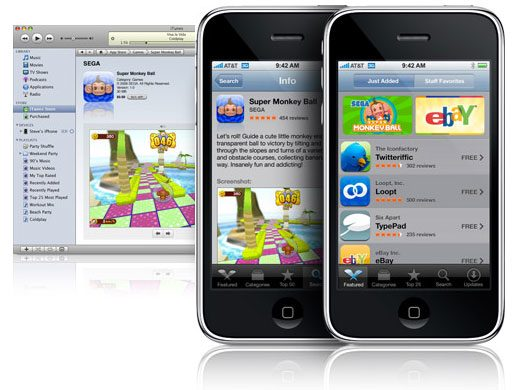
\includegraphics[width=0.7\textwidth]{./img/iOS2-AppStore.jpg}
	\caption{La App Store fue lo más destacado en esta versión, y abrió un nuevo paradigma tanto para el mercado de los smartphones como para los desarrolladores de software.}
\end{figure}

\subsection{iPhone OS 3.0, 17 de junio de 2009}
Presentado durante la conferencia mundial de desarrolladores de Apple de 2009 (WWDC) junto al iPhone 3Gs. Más de 1.000 millones de aplicaciones fueron descargadas desde la aparición de la App Store.

Esta versión trajo funciones tan solicitadas como cortar/copiar y pegar, MMS, y muchas mejoras en las APIs notificaciones \emph{push} para aplicaciones de terceros, acceso a la librería de música, etc.

\begin{figure}[h]
	\centering
		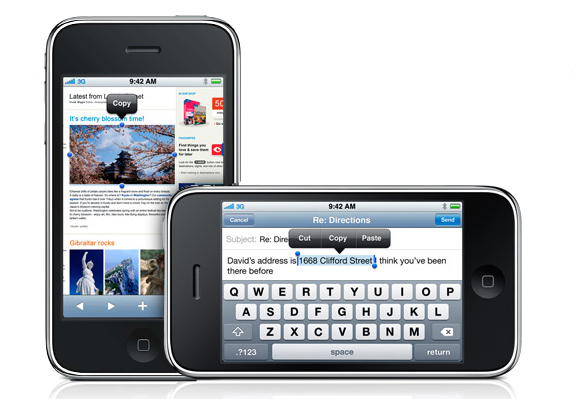
\includegraphics[width=0.7\textwidth]{./img/iOS3.jpg}
	\caption{Ejemplos de copiar y pegar en iPhone OS 3.}
\end{figure}

\subsection{iOS 4, 21 de junio de 2010}
Esta nueva versión trajo diversos cambios significativos al ecosistema de Apple: comenzó a utilizarse la denominación ``iOS'', por primera vez se dejó de dar soporte a ciertos dispositivos (en concreto el iPhone y iPod Touch de 1ª generación) y fue la primera versión que los usuarios de iPod Touch no tuvieron que pagar para actualizar. La actualización 4.2.1 añadió compatibilidad con el iPad.

\subsection{iOS 5, 12 de octubre de 2011}
Coincidiendo con el iPhone 4S, la quinta versión del sistema operativo incorpora novedades como iCloud, Siri, integración con Twitter, iMessage (envío de mensajes via Wi-Fi a otros dispositivos iOS) y mejoras en las notificaciones, entre otros.

Se dejó de dar soporte al iPhone 3G y al iPod Touch de 2ª generación.

Se introduce el concepto de Storyboard, una nueva forma de definir la interfaz de usuario de las aplicaciones iOS. Hasta la fecha, cada \texttt{ViewController} debía llevar un fichero \texttt{.nib} con la interfaz. Un Storyboard es un único fichero que engloba toda la interfaz de usuario del programa, definiendo vistas individuales y las transiciones entre éstas.

Otra gran novedad a nivel de programación es la inclusión del ARC, que elimina la necesidad de llamar explícitamente a métodos para alojar y liberar objetos en memoria.

\begin{figure}[h]
	\centering
		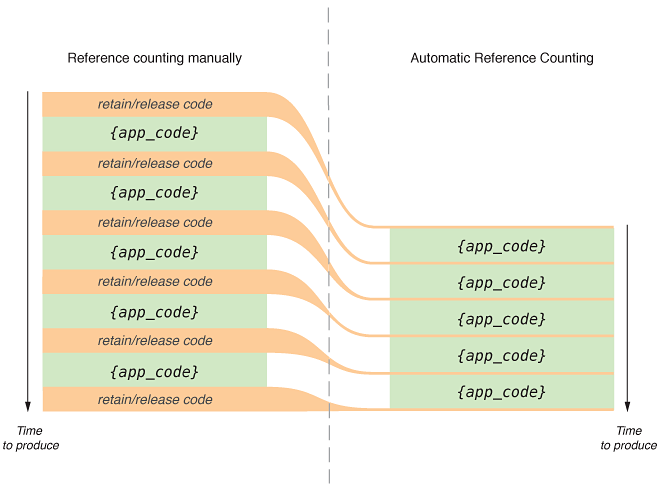
\includegraphics[width=0.7\textwidth]{./img/ARC.png}
	\caption{Reducción de tiempo al escribir código usando ARC.}
\end{figure}

\subsection{iOS 6, 19 de septiembre de 2012}
La sexta versión de iOS deja de dar soporte al iPod Touch de 3ª generación y al iPad de 1ª generación y es lanzada junto al iPhone 5.

iOS 6 fue muy criticado por el público ya que eliminó las aplicaciones Google Maps y Youtube que hasta ahora venían por defecto, forzando así a los usuarios a que usaran la aplicación Maps de Apple, cuya popularidad estaba por los suelos debido a problemas de datos incompletos o inexistentes, sin soporte para transporte público o imágenes de satélite de baja calidad. Apple también tuvo problemas legales ya que la aplicación de reloj generó críticas al ser su interfaz muy parecida al diseño del reloj de las estaciones suizas, marca perteneciente a SBB. Ante estas críticas, Apple accedió a declarar que su diseño estaba influenciado por el de SBB y pagó una tasa por la licencia. \cite{SwissWatch}

Esta fue la última versión en la que Scott Forstall (firme defensor del skeumorfismo) trabajó como vicepresidente de Apple en el departamento de Software de iPhone.

\begin{figure}[h]
	\centering
		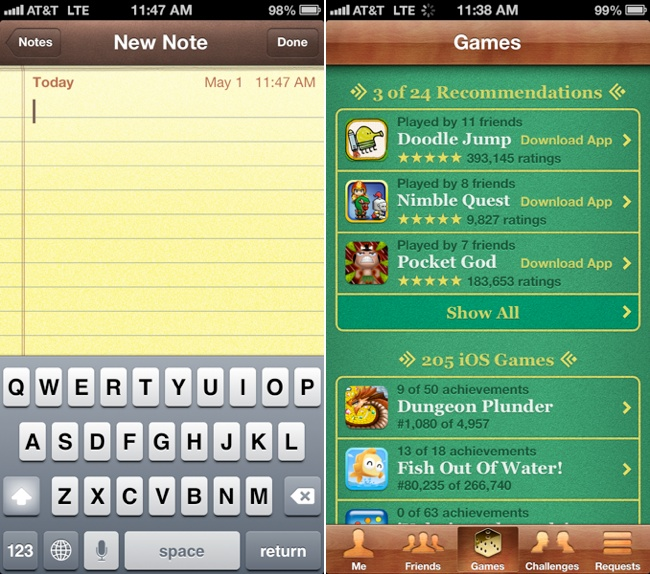
\includegraphics[width=0.7\textwidth]{./img/iOS6-Skeumorphism.jpg}
	\caption{Ejemplos de skeumorfismo, haciendo que el diseño de una aplicación se asemeje a objetos de la realidad.}
\end{figure}

\subsection{iOS 7, 18 de septiembre de 2013}
Con un diseño completamente nuevo (creación del equipo liderado por el vicepresidente senior Sir Jonathan Ive), esta nueva versión traía nuevas funciones como AirDrop, Centro de Control (al hacer swipe desde el borde de abajo de la pantalla), llamadas de solo audio a través de FaceTime y bloqueo remoto en caso de pérdida a través de Find My iPhone.

\begin{figure}[h]
	\centering
		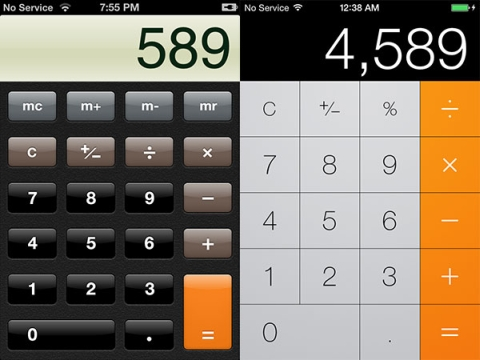
\includegraphics[width=0.7\textwidth]{./img/iOS7-CalculatorRedesign.jpg}
	\caption{Ejemplo del cambio de diseño de la aplicación Calculadora. A la izquierda, la versión en iOS6 (skeumorfismo), y a la derecha la versión de iOS 7 (diseño plano).}
\end{figure}

Se dejó de dar soporte al iPhone 3GS y al iPod Touch de 4ª generación.

\subsection{iOS 8, 7 de septiembre 2014}
Si bien iOS 7 introdujo un cambio en la interfaz, iOS 8 trajo mejoras y nuevas características al sistema operativo móvil de Apple. Fue lanzado junto al iPhone 6 y 6 Plus.

Entre las nuevas características, se puede destacar App Extensions, que permite que una aplicación extienda sus funciones a otras aplicaciones o partes del sistema operativo; autenticación por Touch ID, para poder acceder a las funciones de la API de la lectura de huellas digitales; Metal, una nueva librería destinada al desarrollo de videojuegos; acceso a los frameworks de HealthKit y HomeKit; etc.

En esta nueva versión, el único dispositivo que perdió soporte fue el iPhone 4.

\subsection{iOS 9, 16 de septiembre de 2015}
El sistema operativo madura y sigue introduciendo nuevas características y mejora aspectos que se consideran anticuados (Passbook pasa a llamarse Wallet, la interfaz de cambio de aplicación es completamente nueva, la multitarea se redefine).

Con la llegada del iPhone 6S y 6S Plus, se añade el concepto \textit{3D Touch}, en el que la fuerza con la que se presiona la pantalla con el dedo conlleva acciones distintas. Así, un toque suave genera el gesto ``Peek'', y si se continúa presionando con más fuerza, se accede al gesto ``Pop''. Esto permite realizar acciones o ver contenido sin necesidad de abrir completamente una aplicación, entre otros usos.

Se añaden nuevas APIs para la búsqueda de información dentro de una aplicación. Apple también introduce el concepto ``App Thinning'', para poder reducir el tamaño de una aplicación en los dispositivos (en especial el nuevo Apple TV, que incluye una restricción por aplicación de 200MB) usando sistema de llamada a recursos online bajo demanda.

Esta versión es la única hasta el momento que no deja de dar soporte a ningún dispositivo, por lo que todos los productos que vendía Apple y soportaban iOS 8, también funcionan bajo iOS 9.

\section{Xcode}
Xcode es el IDE por referencia para el desarrollo de software en OS X y iOS. En Xcode se puede programar en C, C++, Objective-C, Objective-C++, Java, Applescript, Python, Ruby, Rez y Swift. El depurador usado en Xcode es LLDB (un set de componentes de LLVM), que reemplazó a GDB desde la versión 4.3.

Xcode incluye las herramientas necesarias para el desarrollo de aplicaciones para OS X, iOS, watchOS y tvOS; desde el editor de código hasta la documentación.

\section{ExpandIT Internet Shop}
Para la realización de este proyecto se necesitaba un proveedor de datos que fuera lo más real posible. Ante la imposibilidad de conseguir acceso al sistema de base de datos de un comercio real, se decidió adaptar una tienda online para el propósito del proyecto.

ExpandIT Internet Shop \cite{EIS} (EIS) es una tienda online desarrollada por la empresa danesa ExpandIT, empresa en la que el autor de este proyecto se encuentra actualmente trabajando de manera remunerada.

EIS es capaz de integrarse con los ERP Microsoft Dynamics NAV (antiguamente conocido como Navision, creado por la empresa danesa PC\&C) o Microsoft Dynamics AX (originalmente desarrollado por IBM y la danesa Damgaard Data como IBM Axapta).

Las modificaciones realizadas al software EIS no son relevantes en este proyecto y no serán descritas, salvo las funciones referentes a la toma y envío de datos por parte del servidor.

\section{JSON}
JSON \cite{JSON} surge como una alternativa mucho más legible para humanos a XML. JSON es actualmente el principal formato usado para la comunicación cliente-servidor asíncrona. Aunque deriva de JavaScript, JSON es un formato independiente de otros lenguajes de programación, lo que permite ser usado por cualquier lenguaje de programación que implemente su generación y parseado.

El esquema seguido por JSON es muy simple, usando parejas de atributos y valores. Los tipos de datos permitidos en JSON son: números, cadenas de caracteres, booleanos, matrices, objetos, y el valor vacío \textit{null}.

\section{Códigos de barras}
El código de barras es una representación de datos de alta densidad relacionada al producto al que va adjunto. Los códigos de barras originales eran de una dimensión, representando los datos por la variación de anchura y espaciado de una serie de líneas paralelas. Posteriormente han evolucionado a matrices de dos dimensiones.

Su uso ha transcendido la compra-venta de productos y son utilizados en cualquier industria, desde el Departamento de Defensa de los Estados Unidos hasta los brazaletes que llevan los pacientes de los hospitales.

Existen multitud de formatos de códigos de barras que son usados en la actualidad. En este proyecto se ha decidido usar el sistema \textit{Code 128}, al ser uno de los más usados en la actualidad y que permite una codificación de caracteres alfanuméricos ASCII (ampliable a caracteres Latin-1).

\begin{figure}[h]
	\centering
		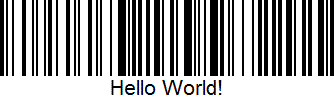
\includegraphics[width=0.7\textwidth]{./img/barcode.png}
	\caption{Código de barras formato Code 128 con el texto ``Hello World!'' codificado.}
\end{figure}

\chapterend